\chapter{Wizualizacja sieci}

Na potrzeby projektu intensywnie poszukiwano metod skutecznego wizualizowania badanych sieci. Przetestowaliśmy większość dostępnych narzędzi, w tym bardzo popularne oprogramowanie Gephi oraz bibliotekę NetworkX. Niestety, ze względu na znaczną wielkość grafów, żadne z łatwo dostępnych narzędzi nie umożliwiało stworzenia ich interaktywnej animacji. W związku z tym zdecydowano się na dwie, uzupełniające się metody.

\section{Graph-tool draw}

Pierwszą z nich jest funkcja rysująca z biblioteki Graph-tool. Posiada ona szerokie możliwości odnośnie formy wyjściowej rysowanych grafów. Okno interaktywne nie zapewniało odpowiedniej płynności animacji, co w praktyce uniemożliwiało korzystanie z niego. Zadowalająca z kolei okazała się możliwość generacji statycznych obrazów PNG w dużej rozdzielczości. Maksymalna rozdzielczość nie była ograniczona przez bibliotekę, z sukcesem generowano obrazy 20 000 x 20 000 pixeli. Jednakże ilość pamięci operacyjnej na dostępnym sprzęcie testowym narzucała ograniczenie na rozdzielczość i w efekcie zdecydowano się na 10 000 x 10 000. Zapewnia to odpowiednią ostrość nawet przy dużym powiększeniu.
 
Funkcja udostępniała kolorowanie grafu i zmianę rozmiarów jego wierzchołków zgodnie z wyliczoną miarą centralności. Kolorowanie odbywało się według skali \textit{gnuplot}, im wartość miary była większa, tym kolor był cieplejszy (bliżej żółtego).

\FloatBarrier\FloatBarrier
\begin{figure}[h]
	\centering
	
\includegraphics[width=\textwidth]{colormaps_reference_05.jpg}
	\caption{Użyta mapa koloru}
\end{figure}
\FloatBarrier\FloatBarrier

Poniżej znajdują się wizualizacje dla wszystkich 3 algorytmów dla najstarszego grafu (1997 rok) oraz najmłodszego (2000 rok).

\FloatBarrier\FloatBarrier
\begin{figure}[h]
	\centering
	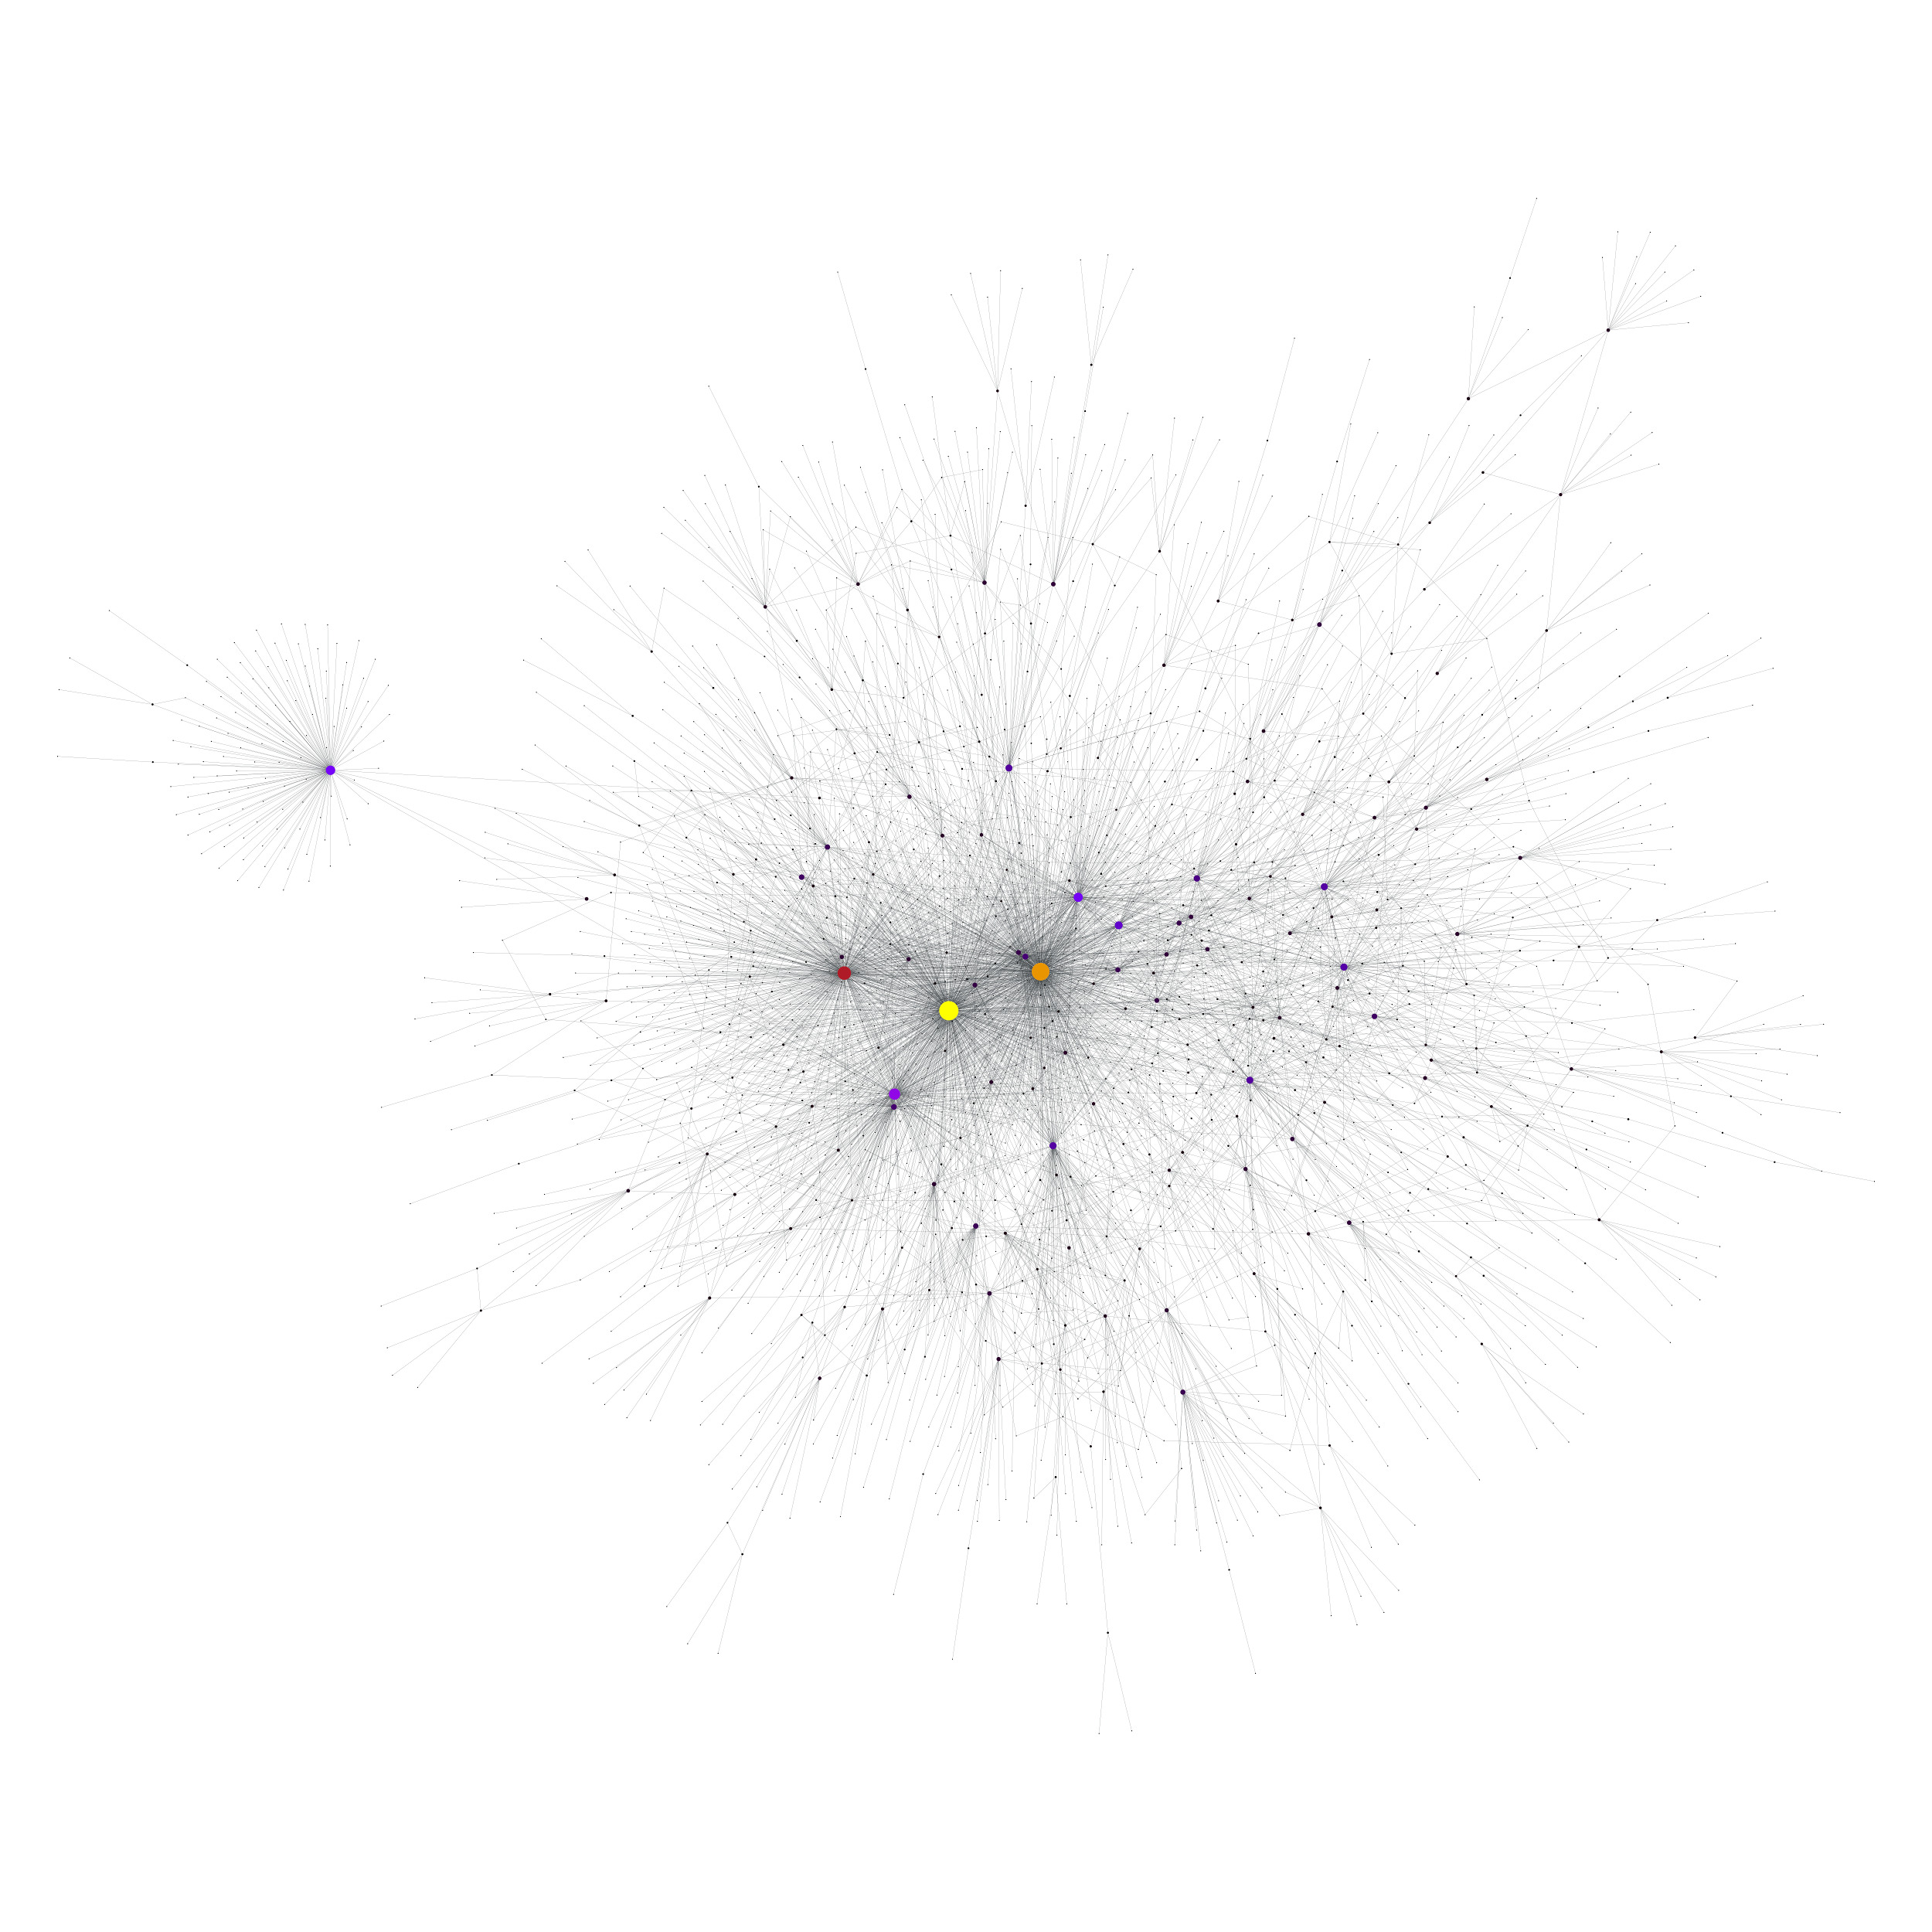
\includegraphics[width=\textwidth]{3015_betweenness.jpg}
	\caption{Graf z początku zebranego zestawu danych dla algorytmu betweenness}
\end{figure}
\FloatBarrier\FloatBarrier

\FloatBarrier\FloatBarrier
\begin{figure}[h]
	\centering
	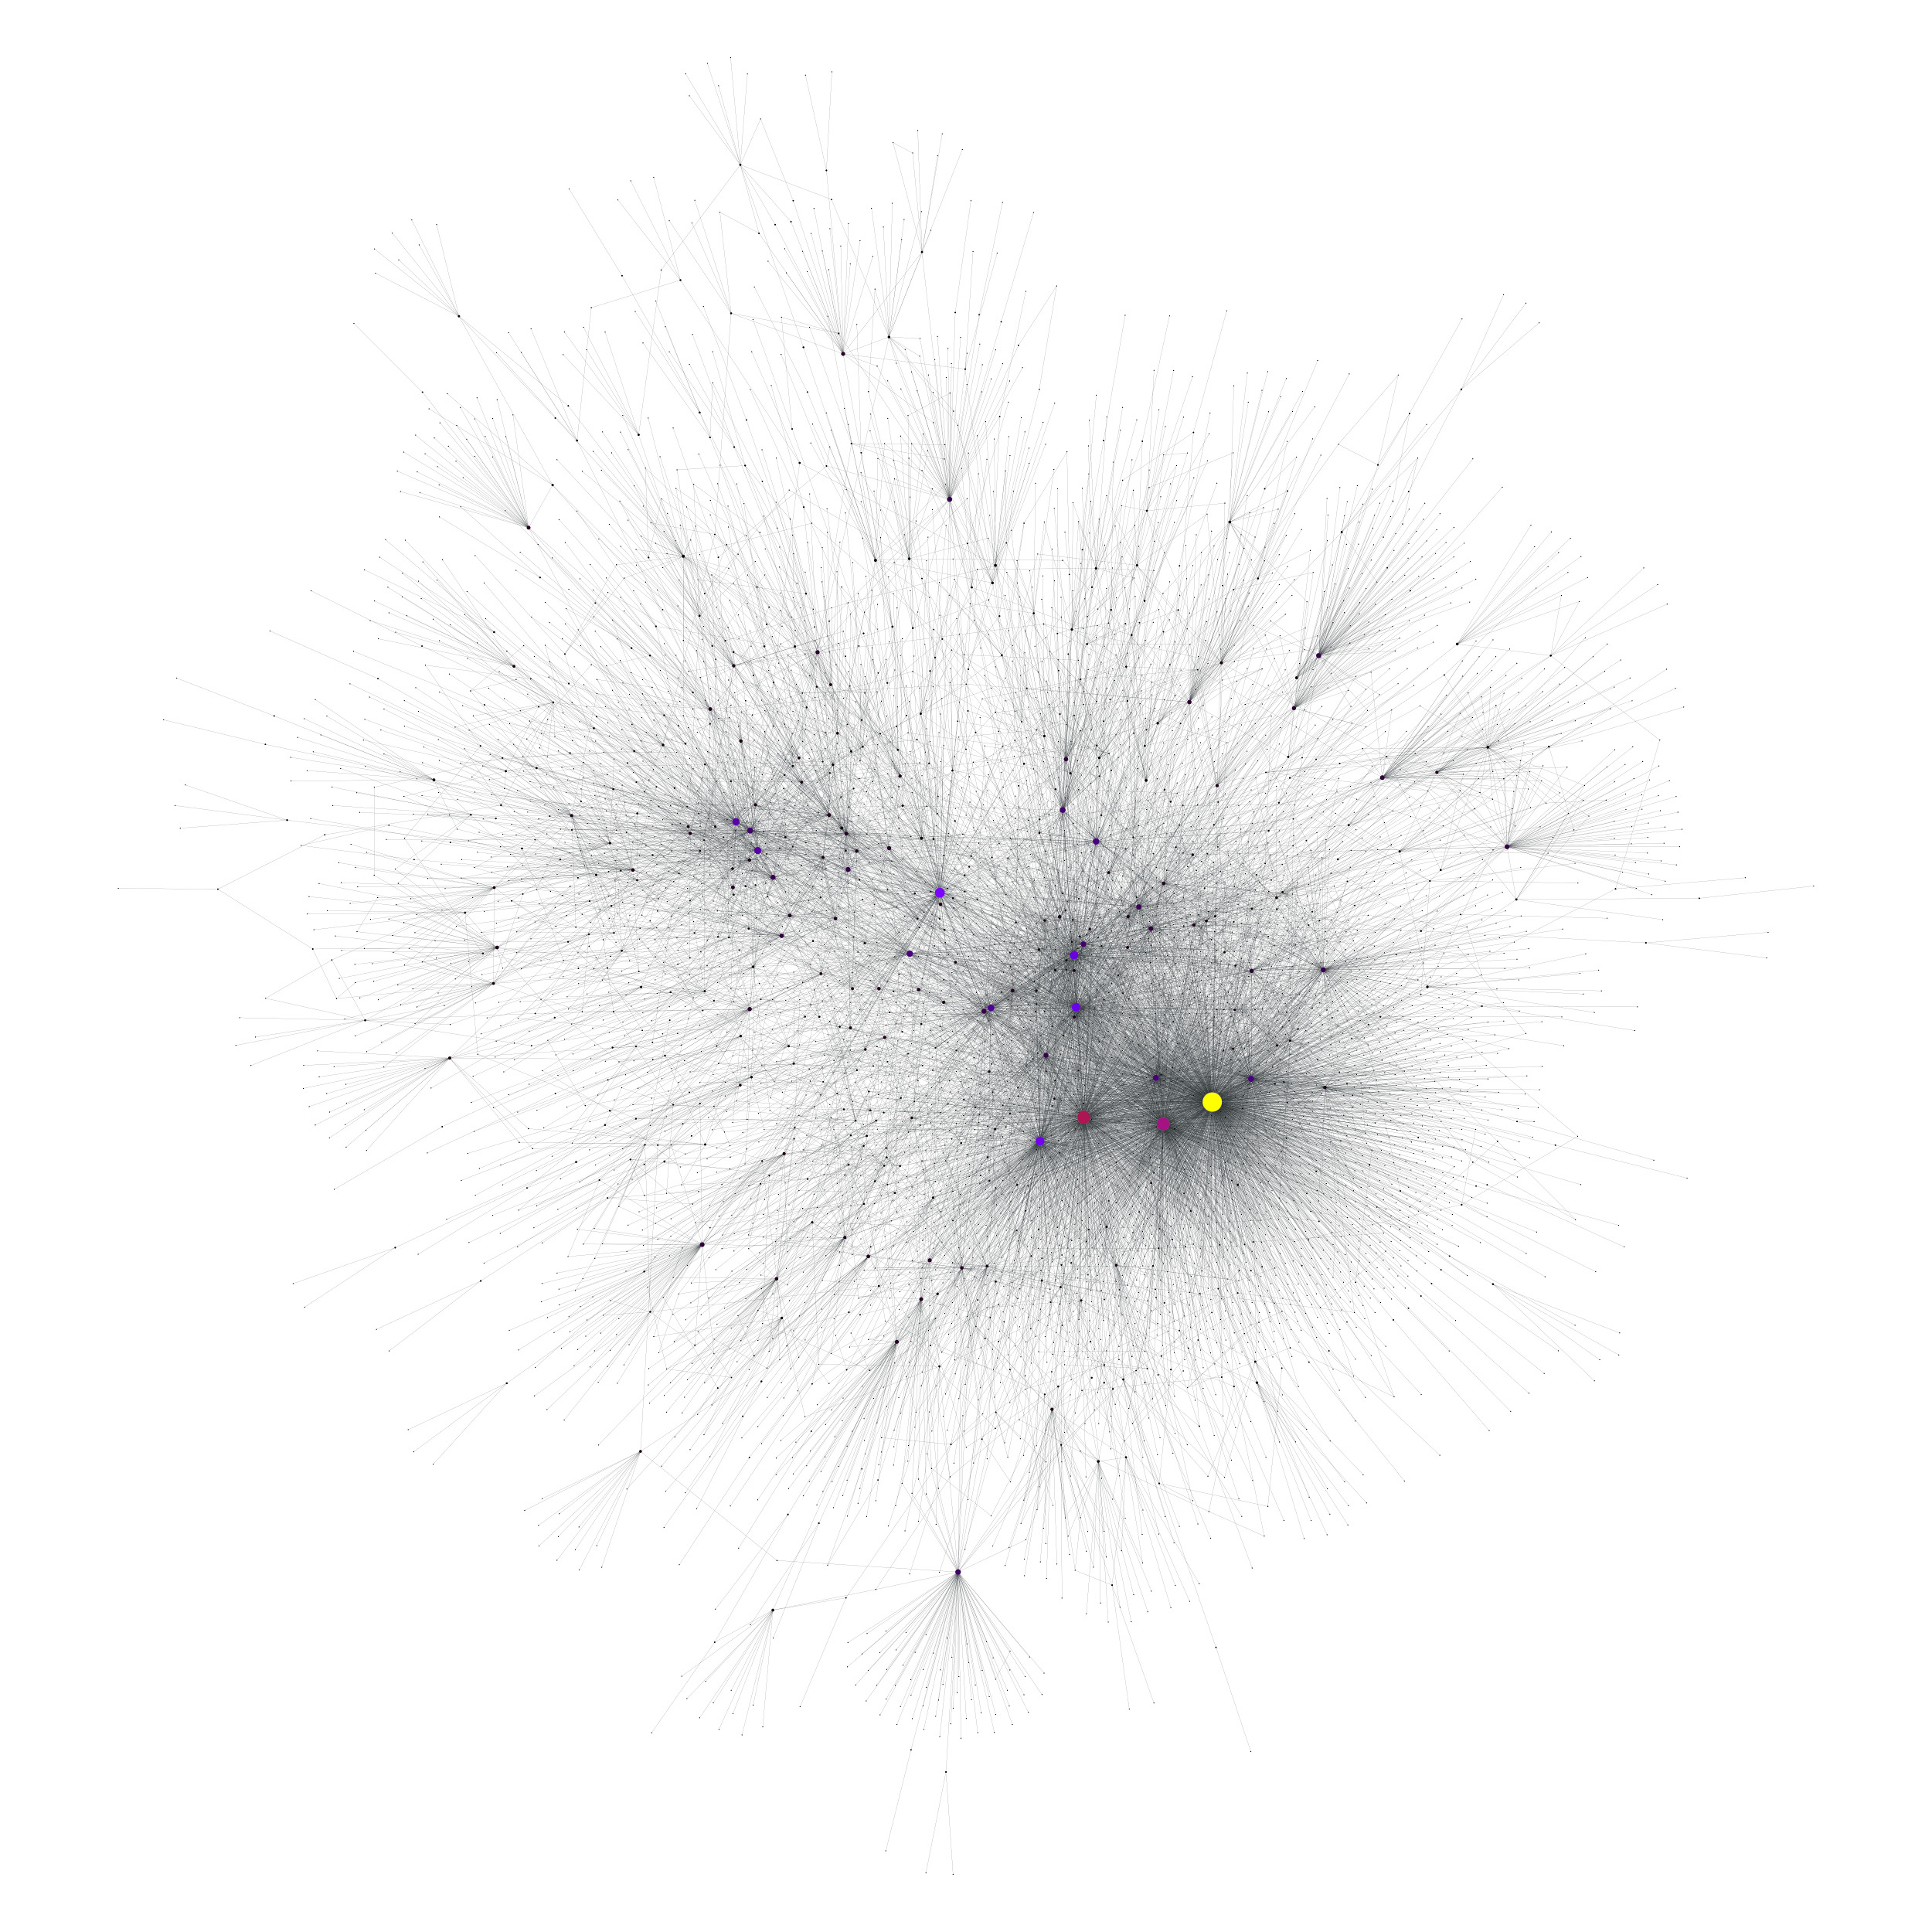
\includegraphics[width=\textwidth]{6474_betweenness.jpg}
	\caption{Graf z końca zebranego zestawu danych dla algorytmu betweenness}
\end{figure}
\FloatBarrier\FloatBarrier

\FloatBarrier\FloatBarrier
\begin{figure}[h]
	\centering
	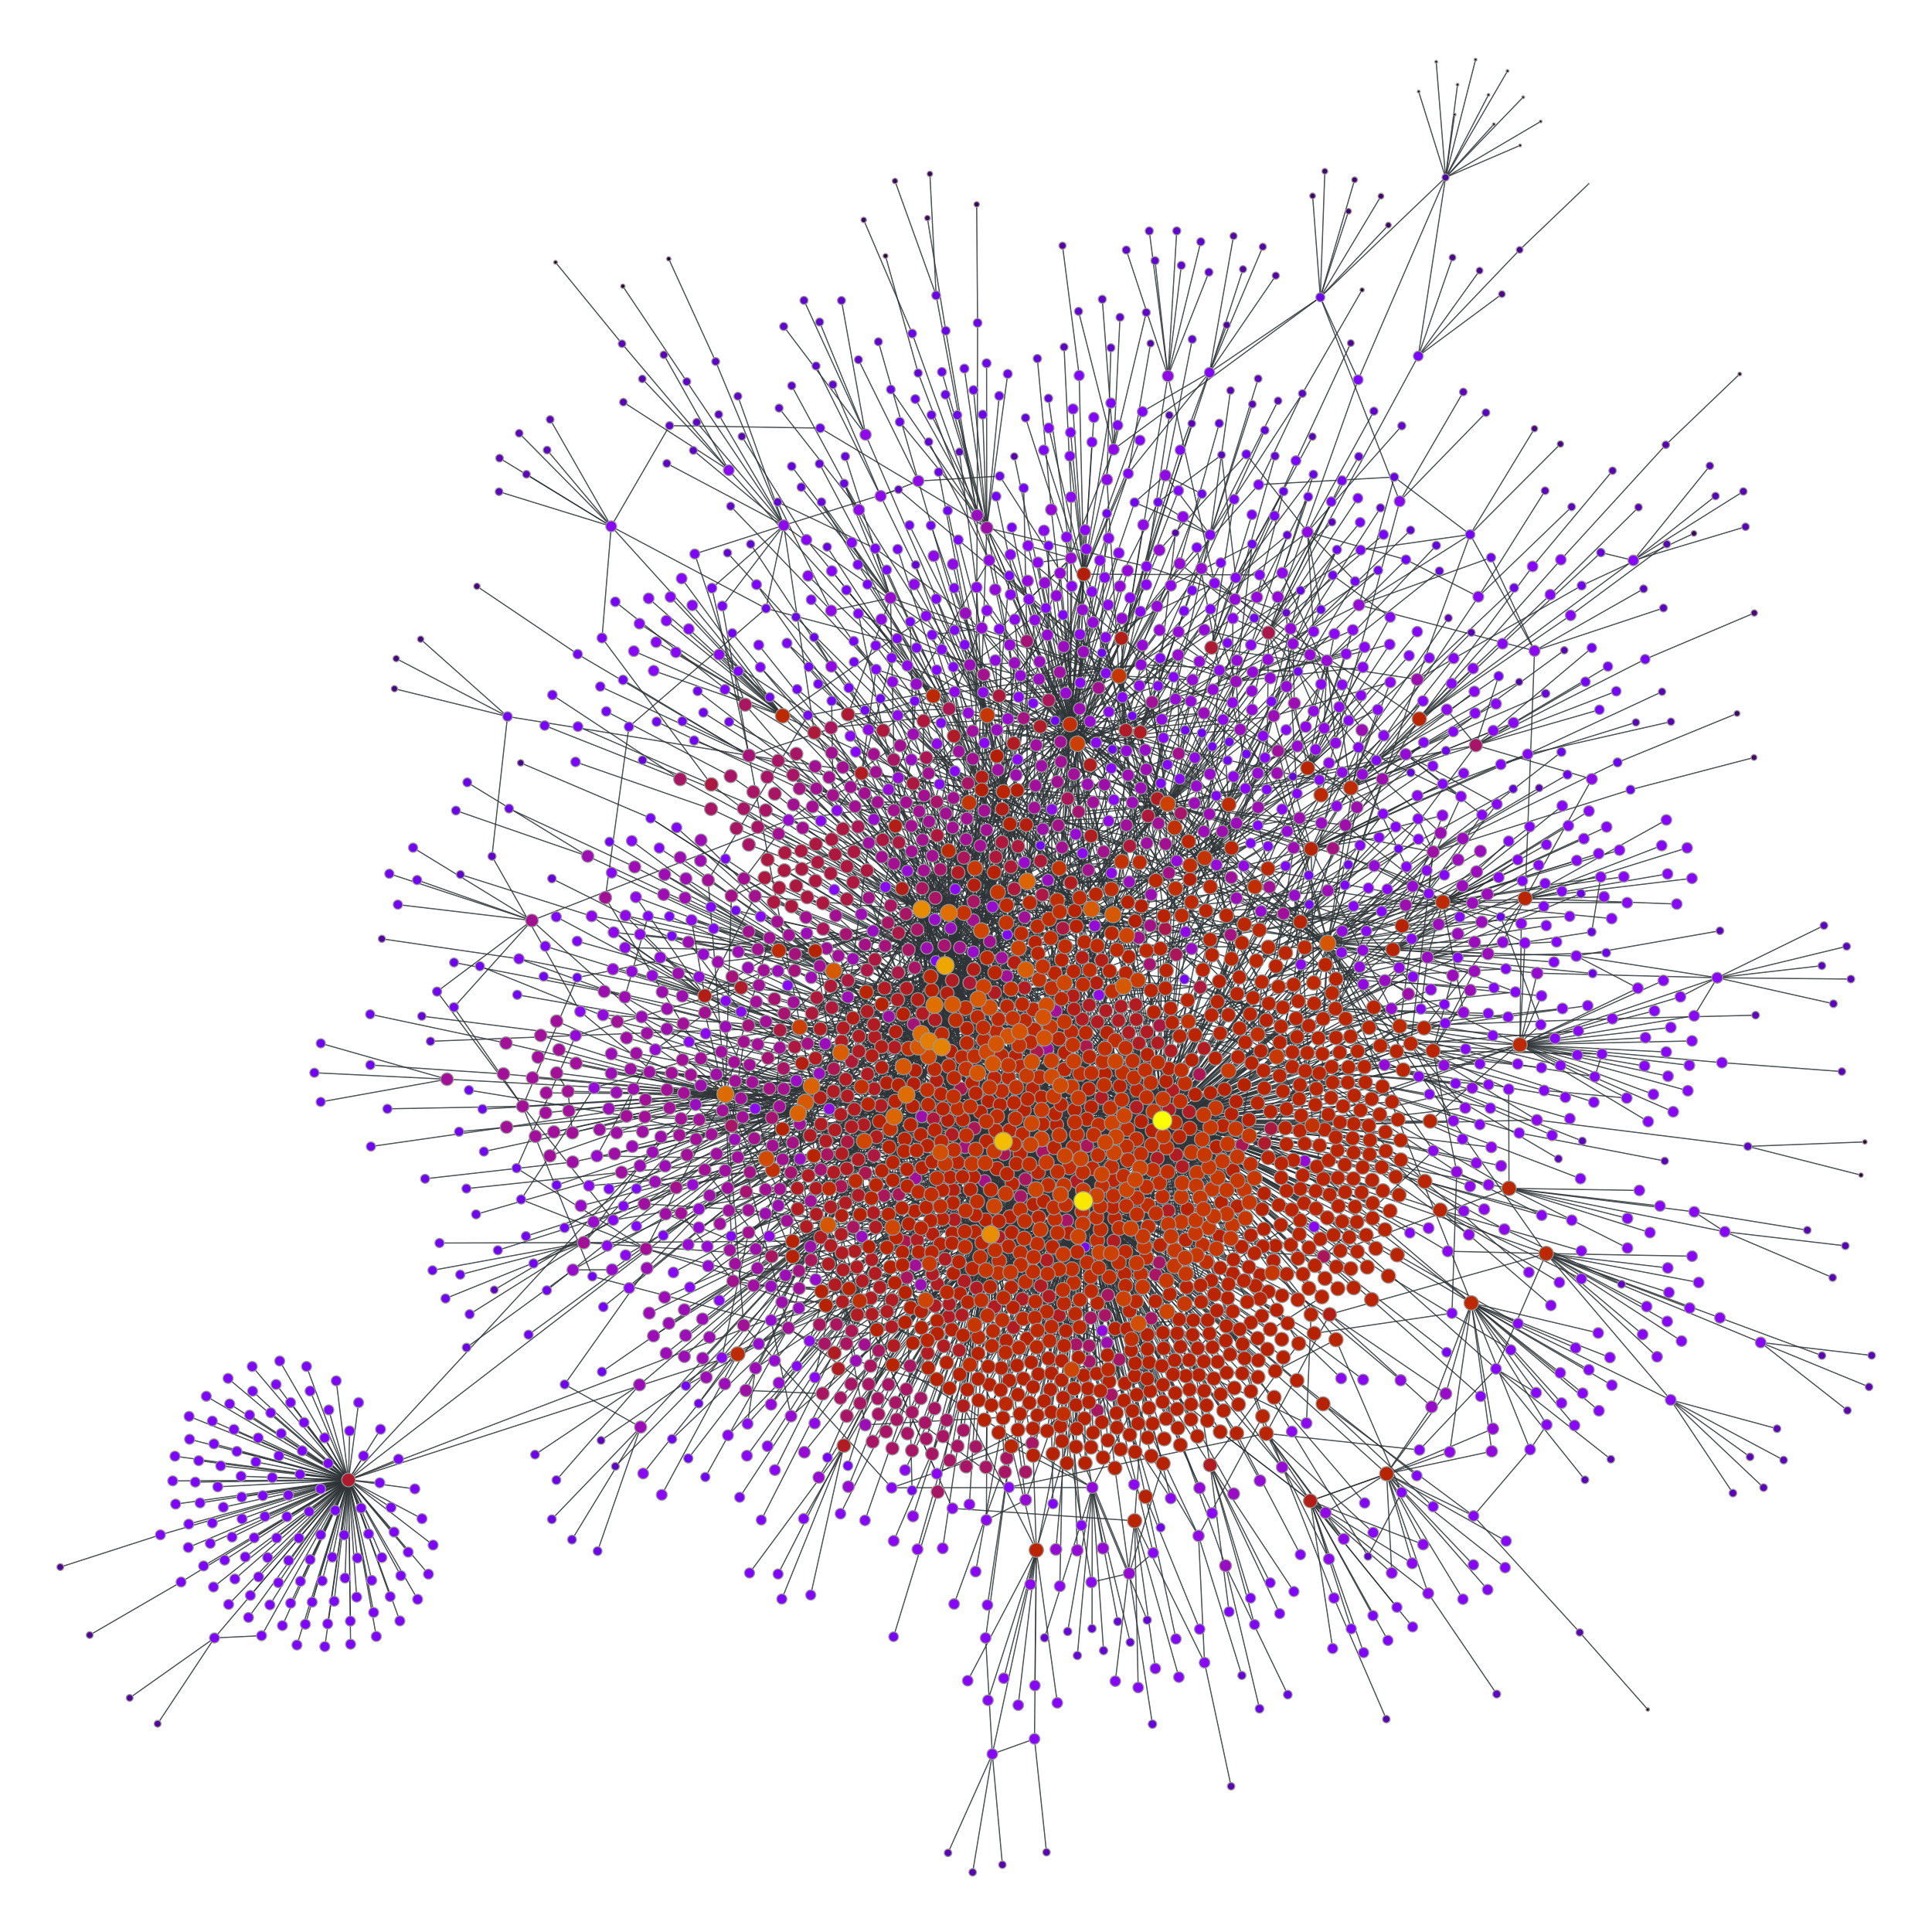
\includegraphics[width=\textwidth]{3015_closeness.jpg}
	\caption{Graf z początku zebranego zestawu danych dla algorytmu closeness}
\end{figure}
\FloatBarrier\FloatBarrier

\FloatBarrier\FloatBarrier
\begin{figure}[h]
	\centering
	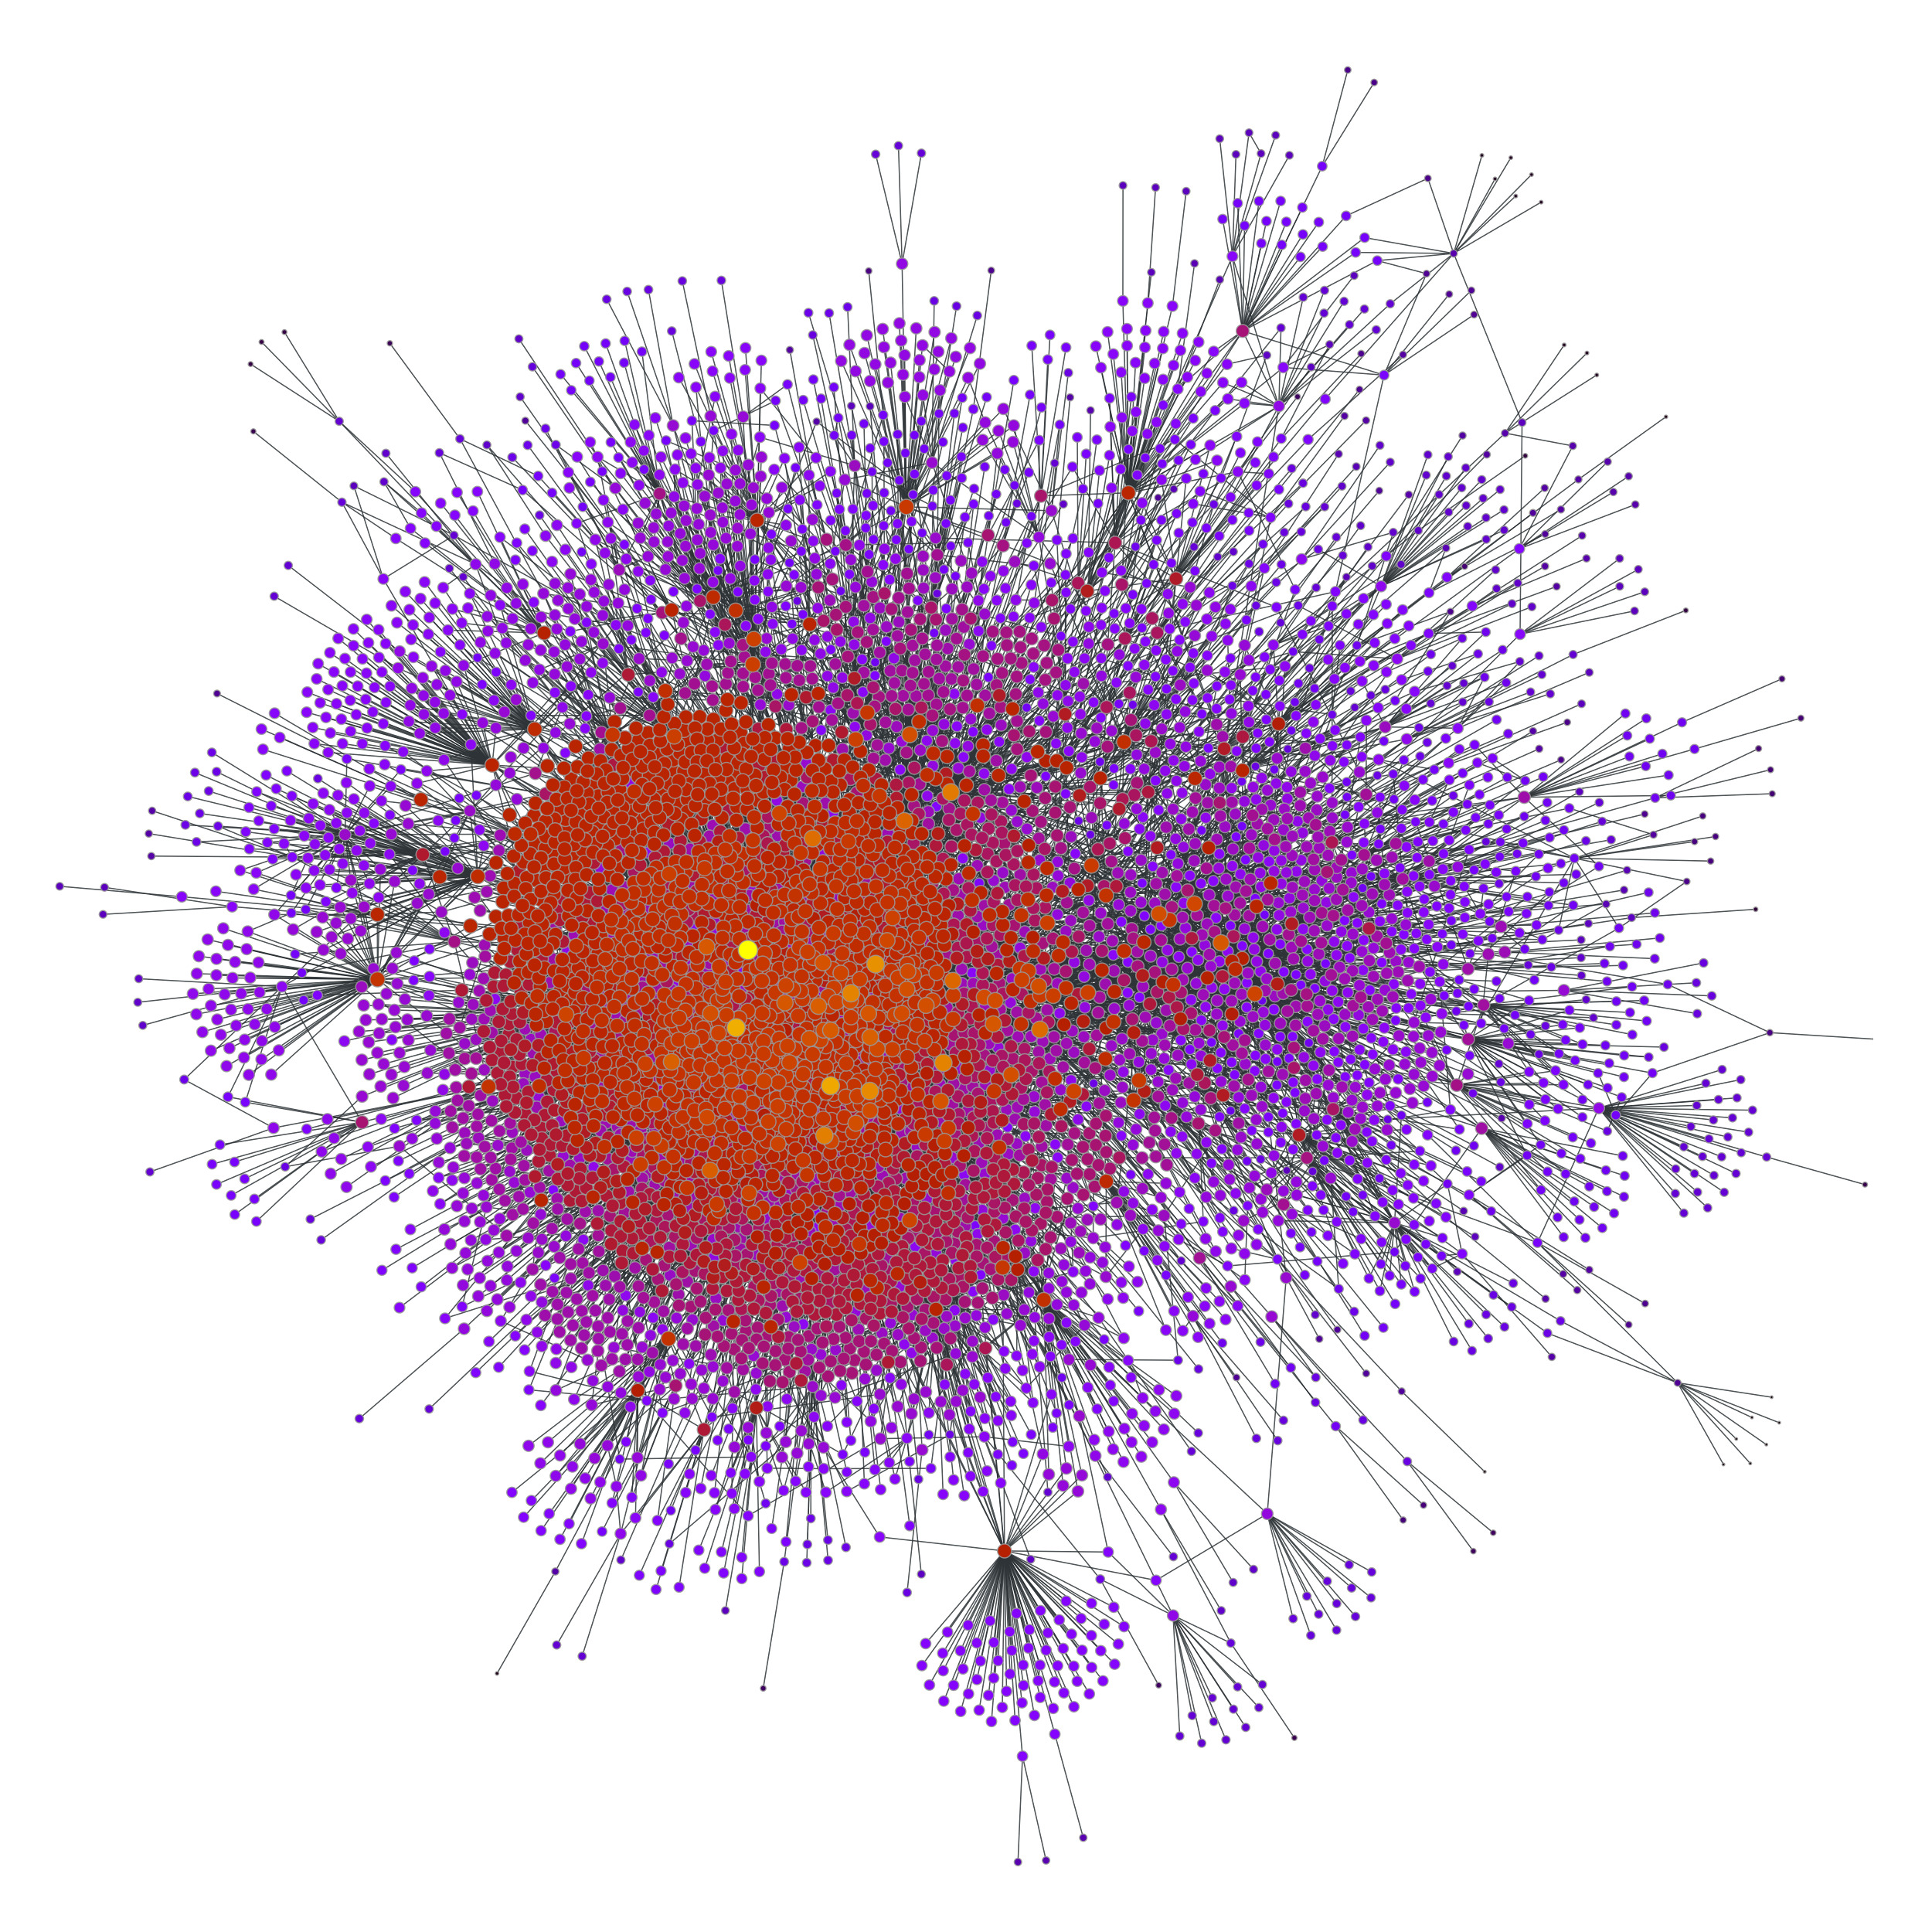
\includegraphics[width=\textwidth]{6474_closeness.jpg}
	\caption{Graf z końca zebranego zestawu danych dla algorytmu closeness}
\end{figure}
\FloatBarrier\FloatBarrier

\FloatBarrier\FloatBarrier
\begin{figure}[h]
	\centering
	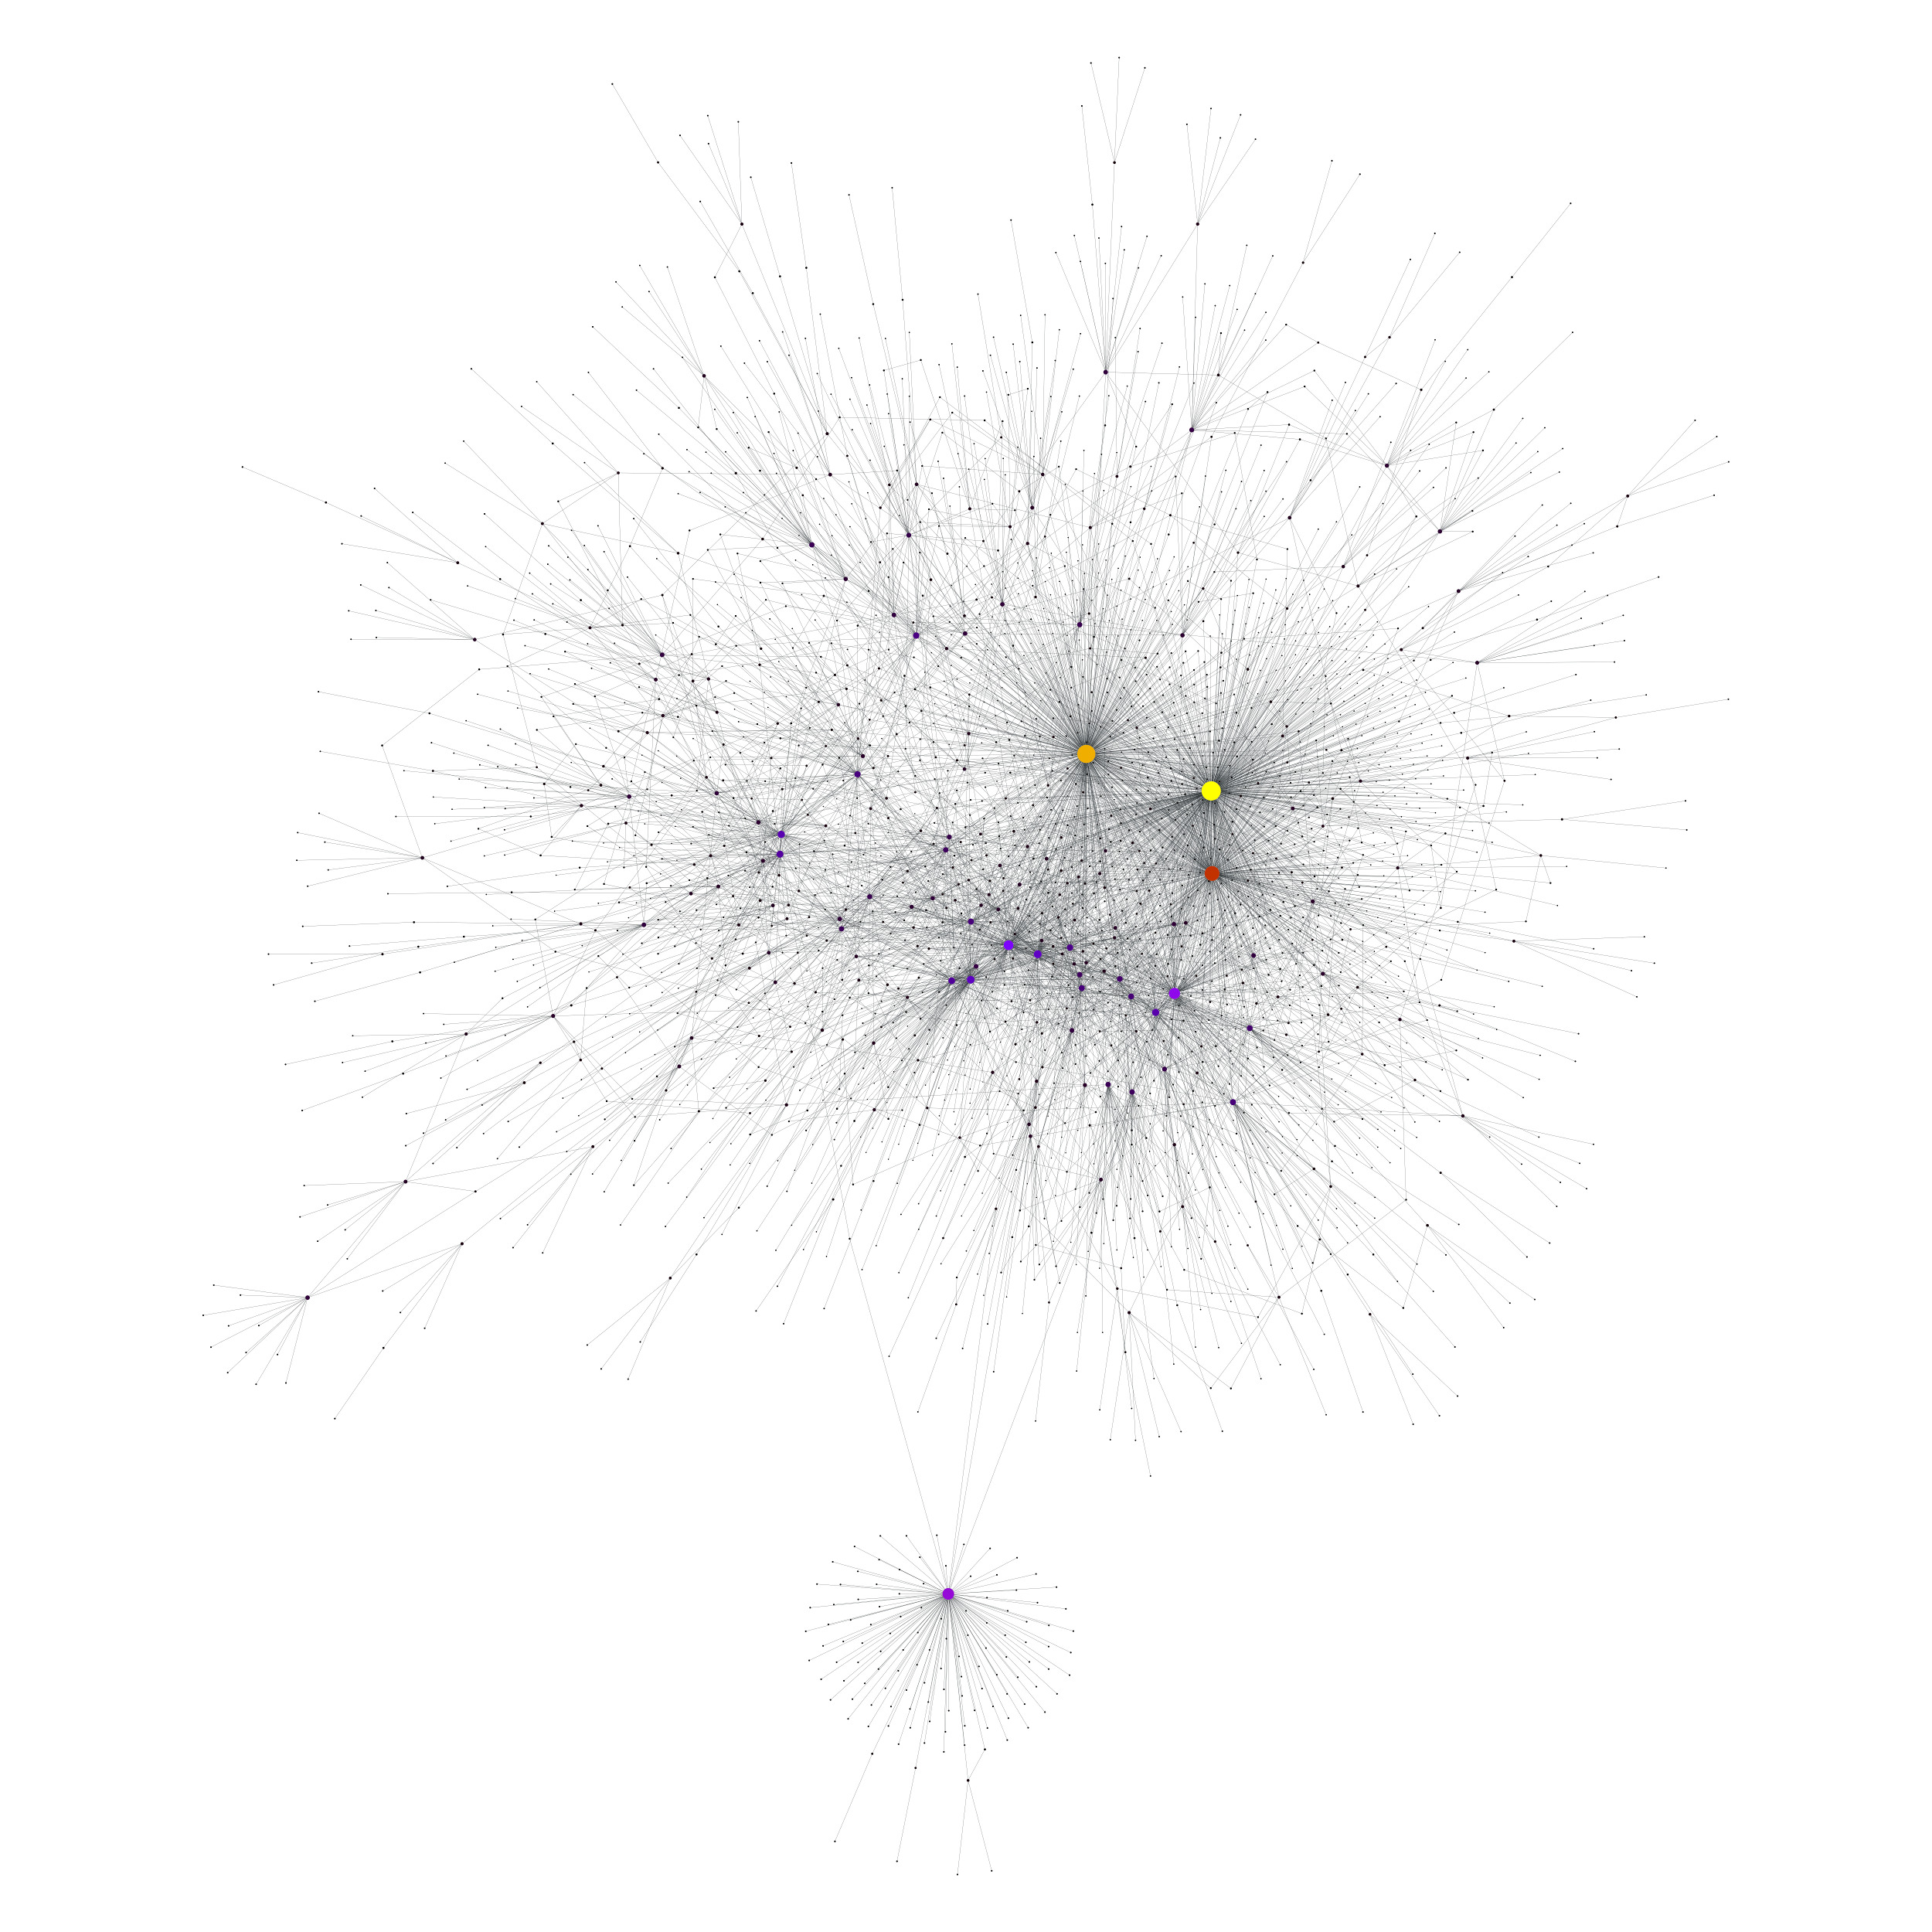
\includegraphics[width=\textwidth]{3015_pagerank.jpg}
	\caption{Graf z początku zebranego zestawu danych dla algorytmu pagerank}
\end{figure}
\FloatBarrier\FloatBarrier

\FloatBarrier\FloatBarrier
\begin{figure}[h]
	\centering
	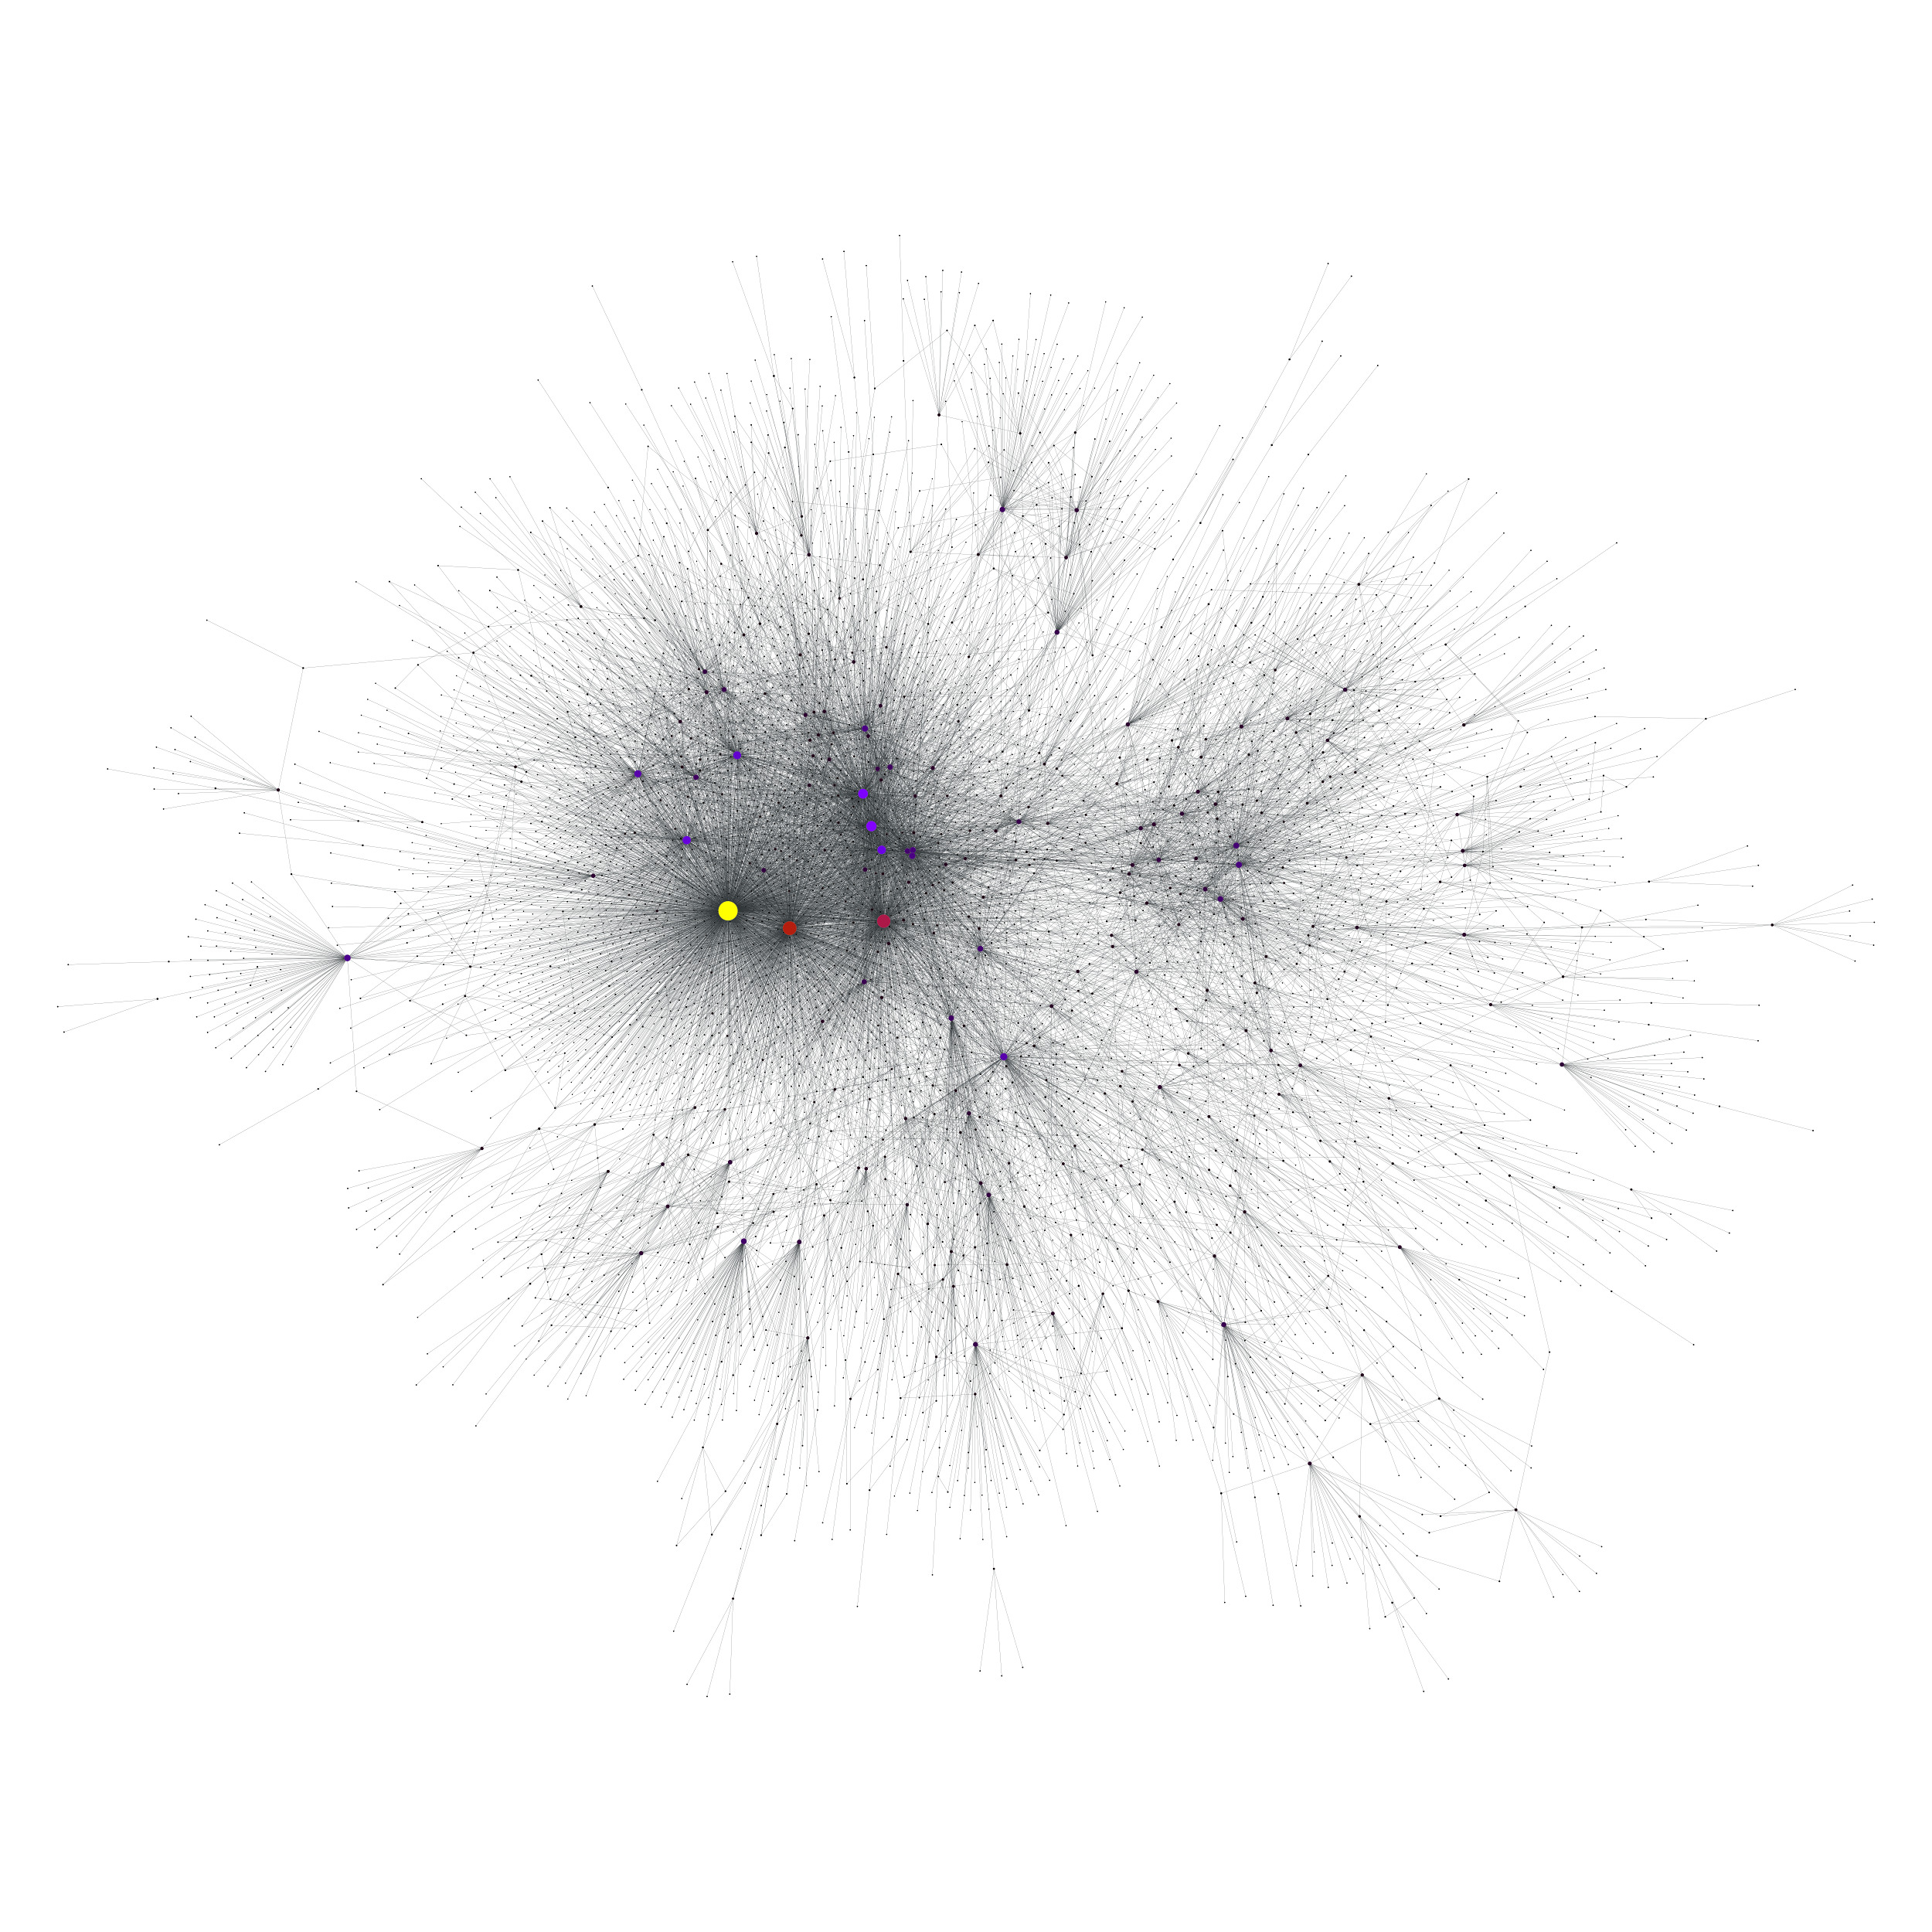
\includegraphics[width=\textwidth]{6474_pagerank.jpg}
	\caption{Graf z końca zebranego zestawu danych dla algorytmu pagerank}
\end{figure}
\FloatBarrier\FloatBarrier

\section{Walrus}

Druga metoda wizualizacji opierała się na oprogramowaniu Walrus, stworzonym w okolicach 2000 roku przez organizację CAIDA, zajmującą się badaniem topologii sieci. Jego rozwój zakończono w 2005 roku, mimo to jest to jedyne narzędzie będące w stanie interaktywnie zwizualizować bardzo duże grafy na stosunkowo słabym sprzęcie i to w przestrzeni trójwymiarowej. Mimo tych niewątpliwych zalet program jest toporny w użytkowaniu i nadaje się głównie do grafów zbliżonych do drzewa rozpinającego. Wymaga on pliku wsadowego w egzotycznym formacie LibSea, konieczne więc było napisanie specjalnego generatora. Do innych ograniczeń zaliczyć można: 
\begin{itemize}
\item obsługa wyłącznie grafów skierowanych
\item obsługa tylko grafów spójnych
\item podanie w pliku wsadowym pełnego drzewa rozpinającego
\item brak obsługi krawędzi wielokrotnych i cykli w grafie
\item brak obsługi pętli w grafie
\end{itemize}

Powyższe ograniczenia wymusiły dokonania transformacji grafu. Efekty widoczne są poniżej. Podobnie jak w pierwszej metodzie, kolory odpowiadają przeskalowanej wartości miar centralności. Kolorowane są również krawędzie, według zasady: krawędź łącząca dwa węzły przyjmuje kolor wierzchołka o większej przypisanej wartości miary. Zdecydowano się na takie rozwiązanie w celu zwiększenia widoczności wierzchołków. Z tego samego powodu poniższe wizualizacje zawierają tylko drzewo spinające badanych grafów. Ostania obejmuje cały graf w celach porównawczych. 

\FloatBarrier\FloatBarrier
\begin{figure}[h]
	\centering
	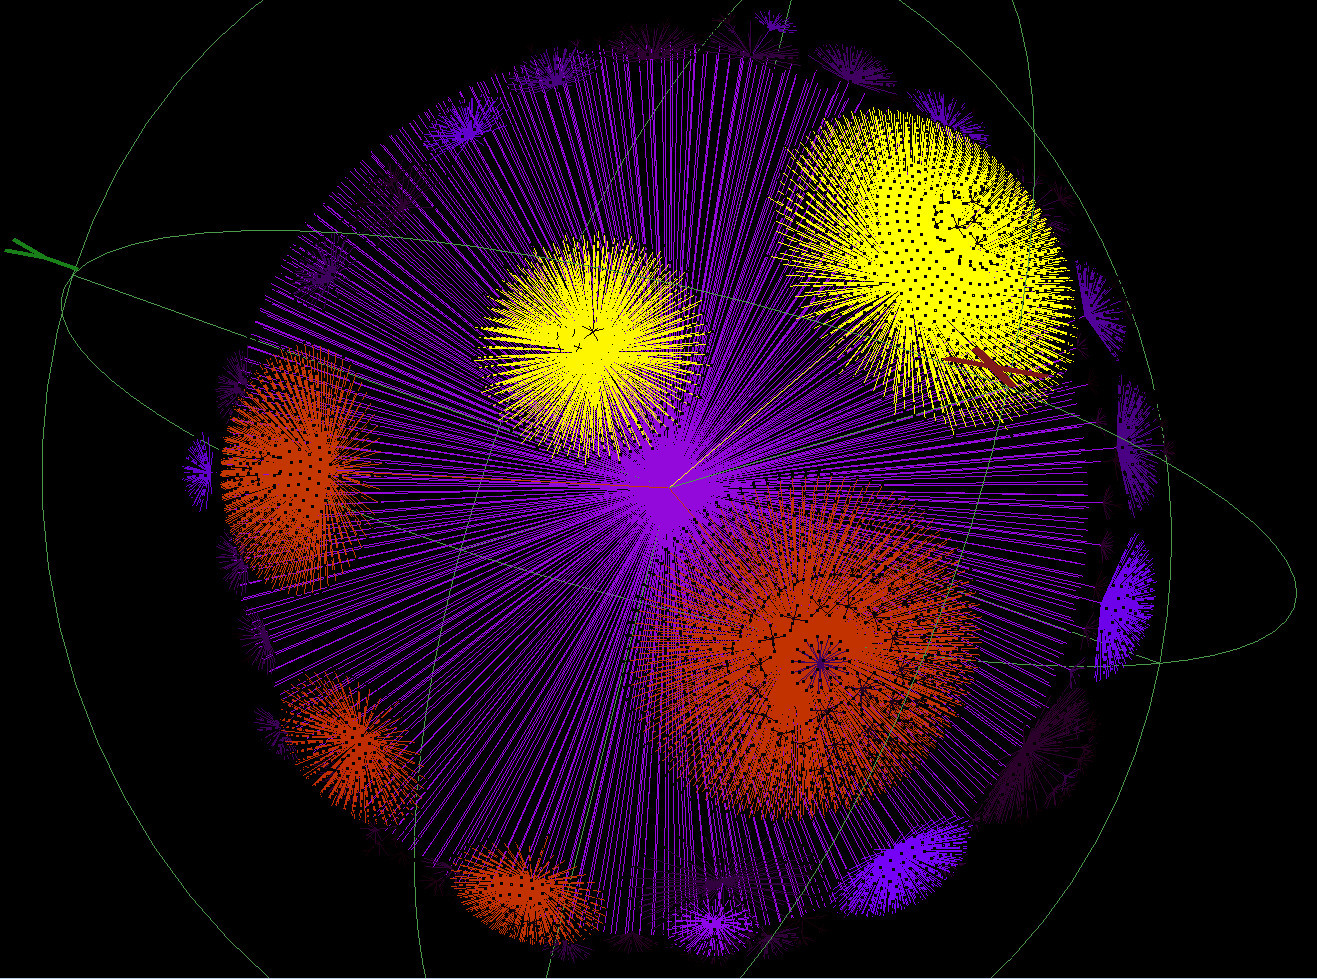
\includegraphics[width=\textwidth]{Betweenness_walrus.jpg}
	\caption{Najstarszy graf, wizualizacja algorytmu betweenness}
\end{figure}
\FloatBarrier\FloatBarrier
\FloatBarrier\FloatBarrier
\begin{figure}[h]
	\centering
	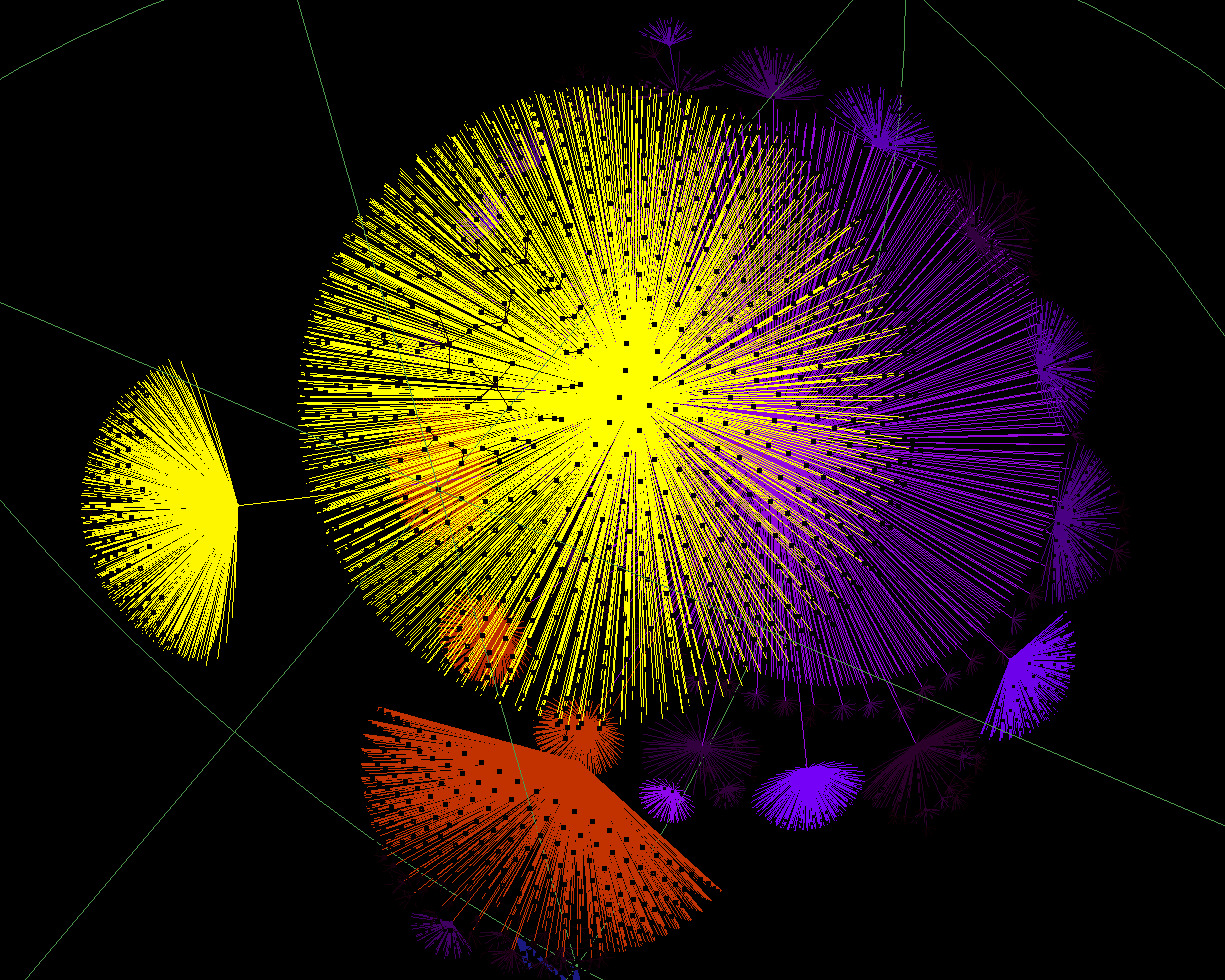
\includegraphics[width=\textwidth]{Betweenness2_walrus.jpg}
	\caption{Najstarszy graf, wizualizacja algorytmu betweenness - ujęcie 2}
\end{figure}
\FloatBarrier\FloatBarrier

\FloatBarrier\FloatBarrier
\begin{figure}[h]
	\centering
	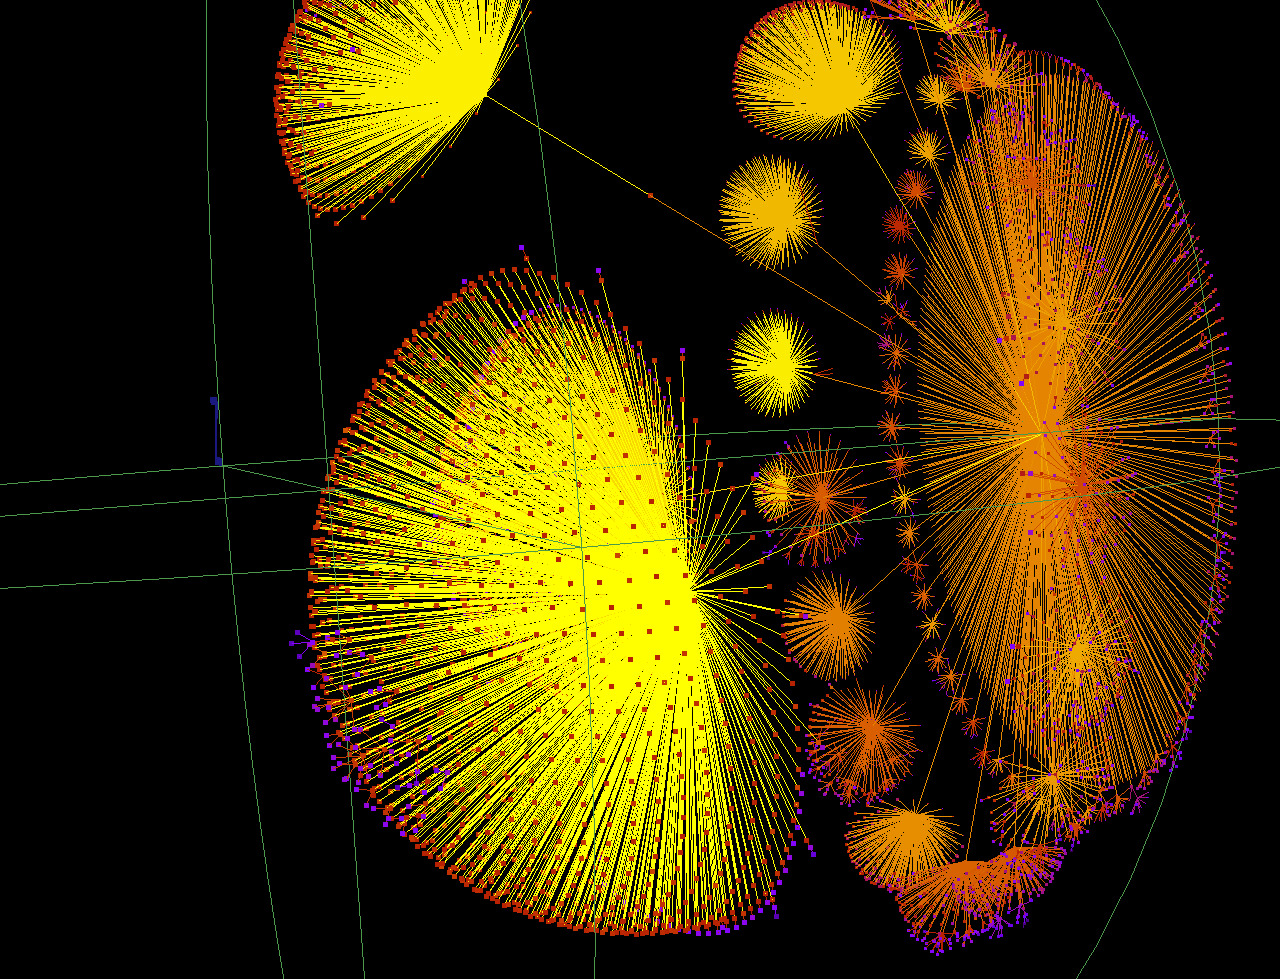
\includegraphics[width=\textwidth]{Closeness_walrus.jpg}
	\caption{Najstarszy graf, wizualizacja algorytmu closeness}
\end{figure}
\FloatBarrier\FloatBarrier
\FloatBarrier\FloatBarrier
\begin{figure}[h]
	\centering
	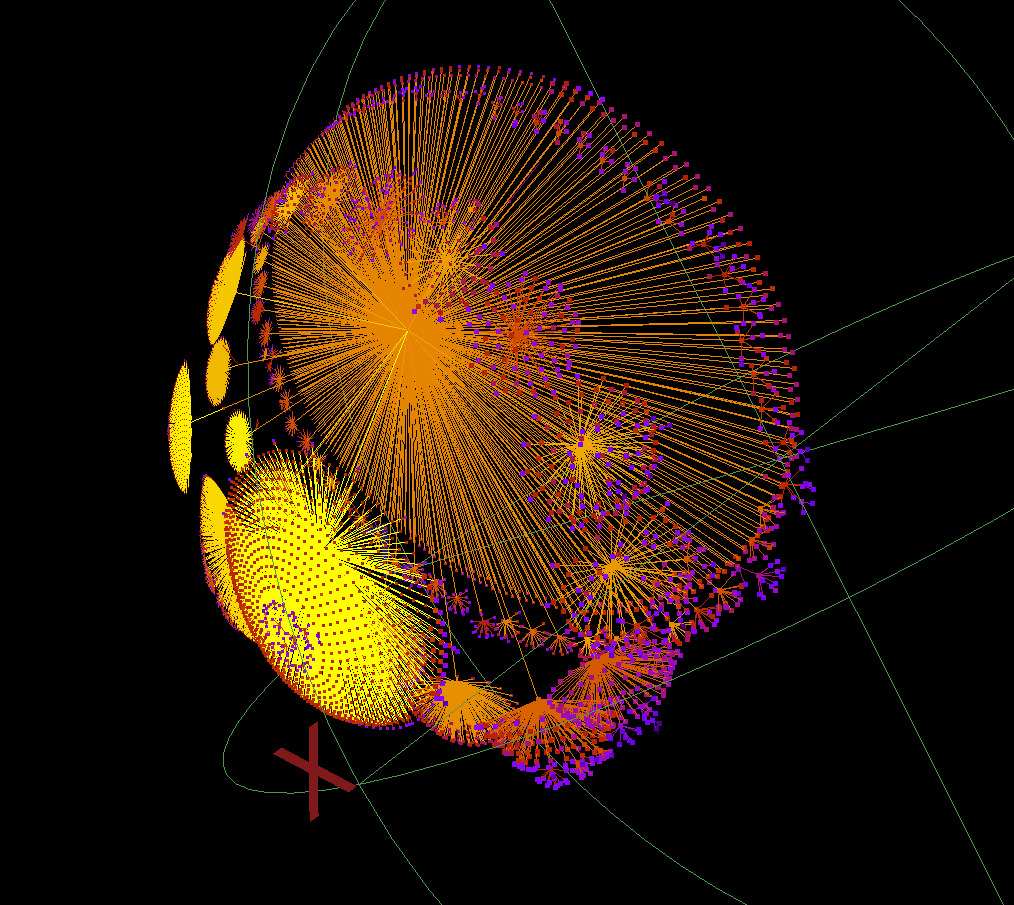
\includegraphics[width=\textwidth]{Closeness2_walrus.jpg}
	\caption{Najstarszy graf, wizualizacja algorytmu closeness - ujęcie 2}
\end{figure}
\FloatBarrier\FloatBarrier        
\FloatBarrier\FloatBarrier
\begin{figure}[h]
	\centering
	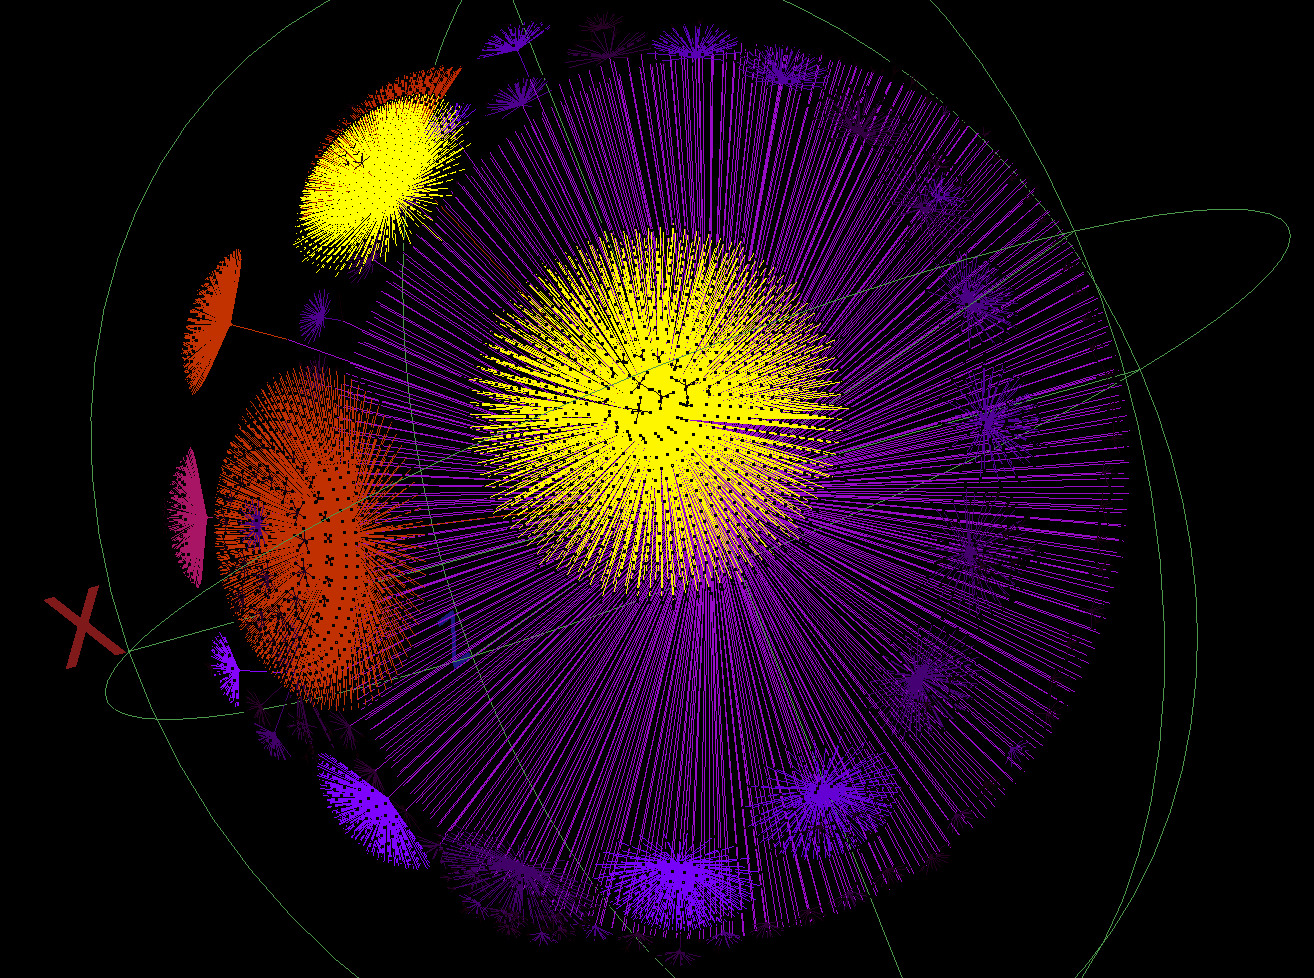
\includegraphics[width=\textwidth]{Pagerank_walrus.jpg}
	\caption{Najstarszy graf, wizualizacja algorytmu pagerank}
\end{figure}
\FloatBarrier\FloatBarrier
\FloatBarrier\FloatBarrier
\begin{figure}[h]
	\centering
	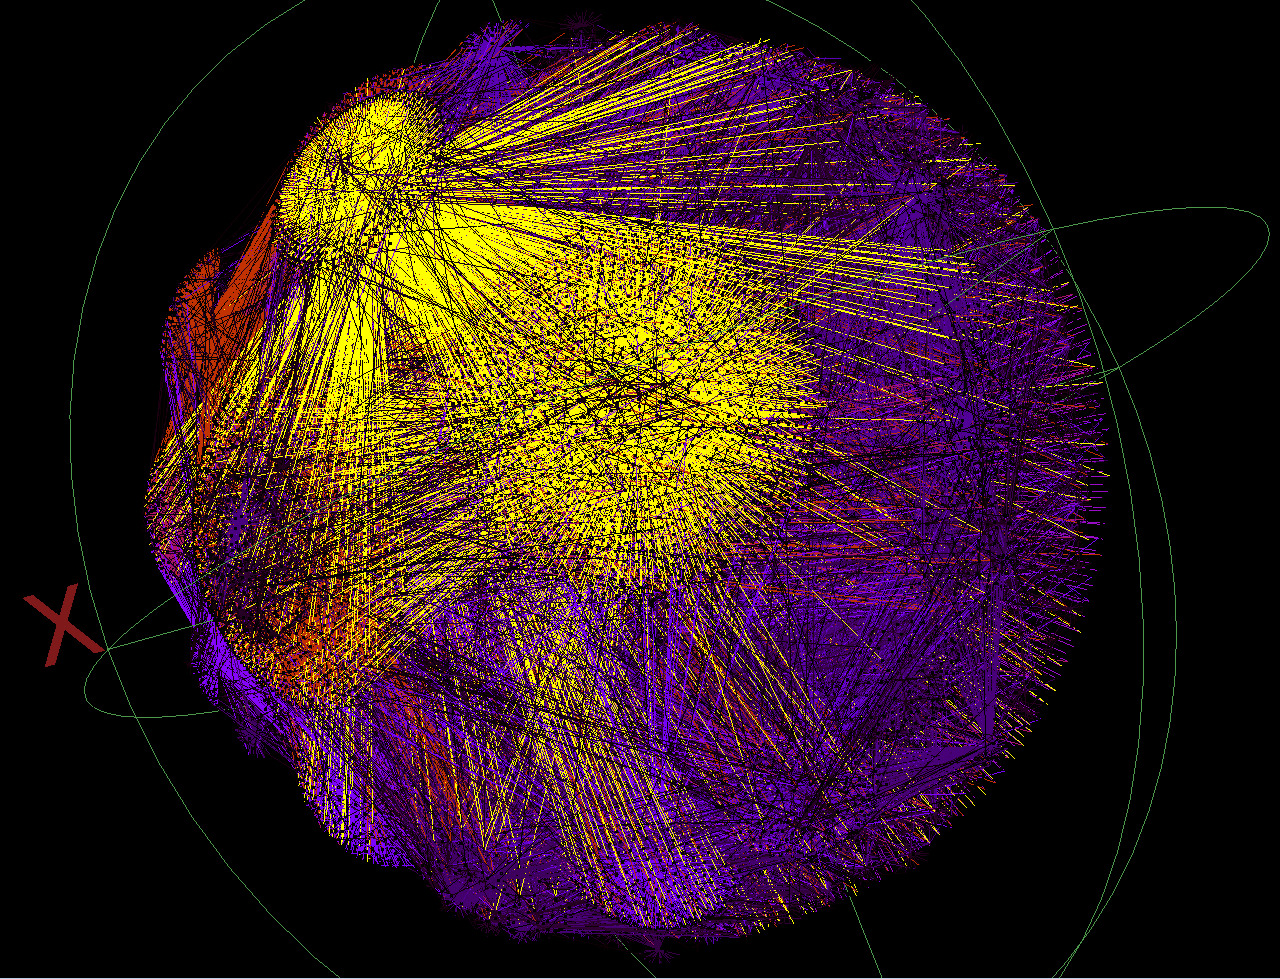
\includegraphics[width=\textwidth]{Pagerank2_walrus.jpg}
	\caption{Najstarszy graf, wizualizacja algorytmu pagerank - cały graf}
\end{figure}
  

Na powyższej ilustracji doskonale widać ogrom badanego grafu. Tak duża liczba krawędzi powoduje, że z wizualizacji ciężko cokolwiek wyczytać. Stąd rezygnacja z części z nich w pozostałych obrazach.